\documentclass[12pt, a4paper, oneside]{book}
\usepackage[hidelinks]{hyperref}
\usepackage[slovak]{babel}
\usepackage{epsfig}
\usepackage{epstopdf}
\usepackage[chapter]{algorithm}
\usepackage{algorithmic}
\usepackage{listings}
\usepackage{amsmath}
\usepackage{amssymb}
\usepackage{graphicx}
\usepackage{multirow}
\usepackage{color}
\usepackage{url}
\usepackage[utf8]{inputenc}
\usepackage[T1]{fontenc}
\usepackage{setspace}
\usepackage{tabularx}
\usepackage{textcomp}
\usepackage{caption}
\usepackage{natbib}
\usepackage{pdfpages}

\setstretch{1.5}
%\renewcommand\baselinestretch{1.5} % riadkovanie jeden a pol

% pekne pokope definujeme potrebne udaje
\newcommand\mftitle{Vývoj softvéru na plánovanie kozmického odpadu pozorovaného jedným a viacerými senzormi}
\newcommand\mfthesistype{Diplomová práca}
\newcommand\mfauthor{Bc. Rastislav Stankovič}
\newcommand\mfadvisor{Mgr. Jiří Šilha, PhD}

\newcommand\mfconsultant{prof. RNDr. Roman Ďurikovič, PhD.}
\newcommand\mfplacedate{Bratislava, 2020}
\newcommand\mfuniversity{UNIVERZITA KOMENSKÉHO V BRATISLAVE}
\newcommand\mffaculty{FAKULTA MATEMATIKY, FYZIKY A INFORMATIKY}
\newcommand{\sub}[1]{$_{\text{#1}}$}
\newcommand{\reference}[1]{č.~\ref{#1}}
\newcommand{\imageHeight}{150px}
\ifx\pdfoutput\undefined\relax\else\pdfinfo{ /Title (\mftitle) /Author (\mfauthor) /Creator (PDFLaTeX) } \fi
\begin{document}

\frontmatter

\thispagestyle{empty}

\noindent
\begin{minipage}{\textwidth}
\begin{center}
\textbf{\mfuniversity \\
\mffaculty}
\end{center}
\end{minipage}

\vfill
\begin{figure}[!hbt]
	\begin{center}
		
\includegraphics{images/logo_fmph}
		\label{img:logo}
	\end{center}
\end{figure}
\begin{center}
	\begin{minipage}{0.8\textwidth}
		\centerline{\textbf{\Large\MakeUppercase{Vývoj softvéru na plánovanie}}}
		\centerline{\textbf{\Large\MakeUppercase{kozmického odpadu pozorovaného}}}
                      \centerline{\textbf{\Large\MakeUppercase{jedným a viacerými senzorm}}}
		\smallskip
		\centerline{\mfthesistype}
	\end{minipage}
\end{center}
\vfill
2020 \hfill
\mfauthor
\eject 
% koniec obalu

\thispagestyle{empty}

\noindent
\begin{minipage}{\textwidth}
\begin{center}
\textbf{\mfuniversity \\
\mffaculty}
\end{center}
\end{minipage}

\vfill
\begin{figure}[!hbt]
\begin{center}

\includegraphics{images/logo_fmph_dark}
\label{img:logo_dark}
\end{center}
\end{figure}
\begin{center}
\begin{minipage}{0.8\textwidth}
		\centerline{\textbf{\Large\MakeUppercase{Vývoj softvéru na plánovanie}}}
		\centerline{\textbf{\Large\MakeUppercase{kozmického odpadu pozorovaného}}}
                      \centerline{\textbf{\Large\MakeUppercase{jedným a viacerými senzorm}}}
\smallskip
\centerline{\mfthesistype}
\end{minipage}
\end{center}
\vfill
\begin{tabular}{l l}
Študijný program: & Aplikovaná informatika\\
Študijný odbor: & 2511 Aplikovaná informatika\\
Školiace pracovisko: & Katedra aplikovanej informatiky\\
Školiteľ: & \mfadvisor \\
Konzultant: & prof. RNDr. Roman Ďurikovič, PhD
\end{tabular}
\vfill
\noindent
\mfplacedate \hfill
\mfauthor
\eject 
% koniec titulneho listu
\thispagestyle{empty}




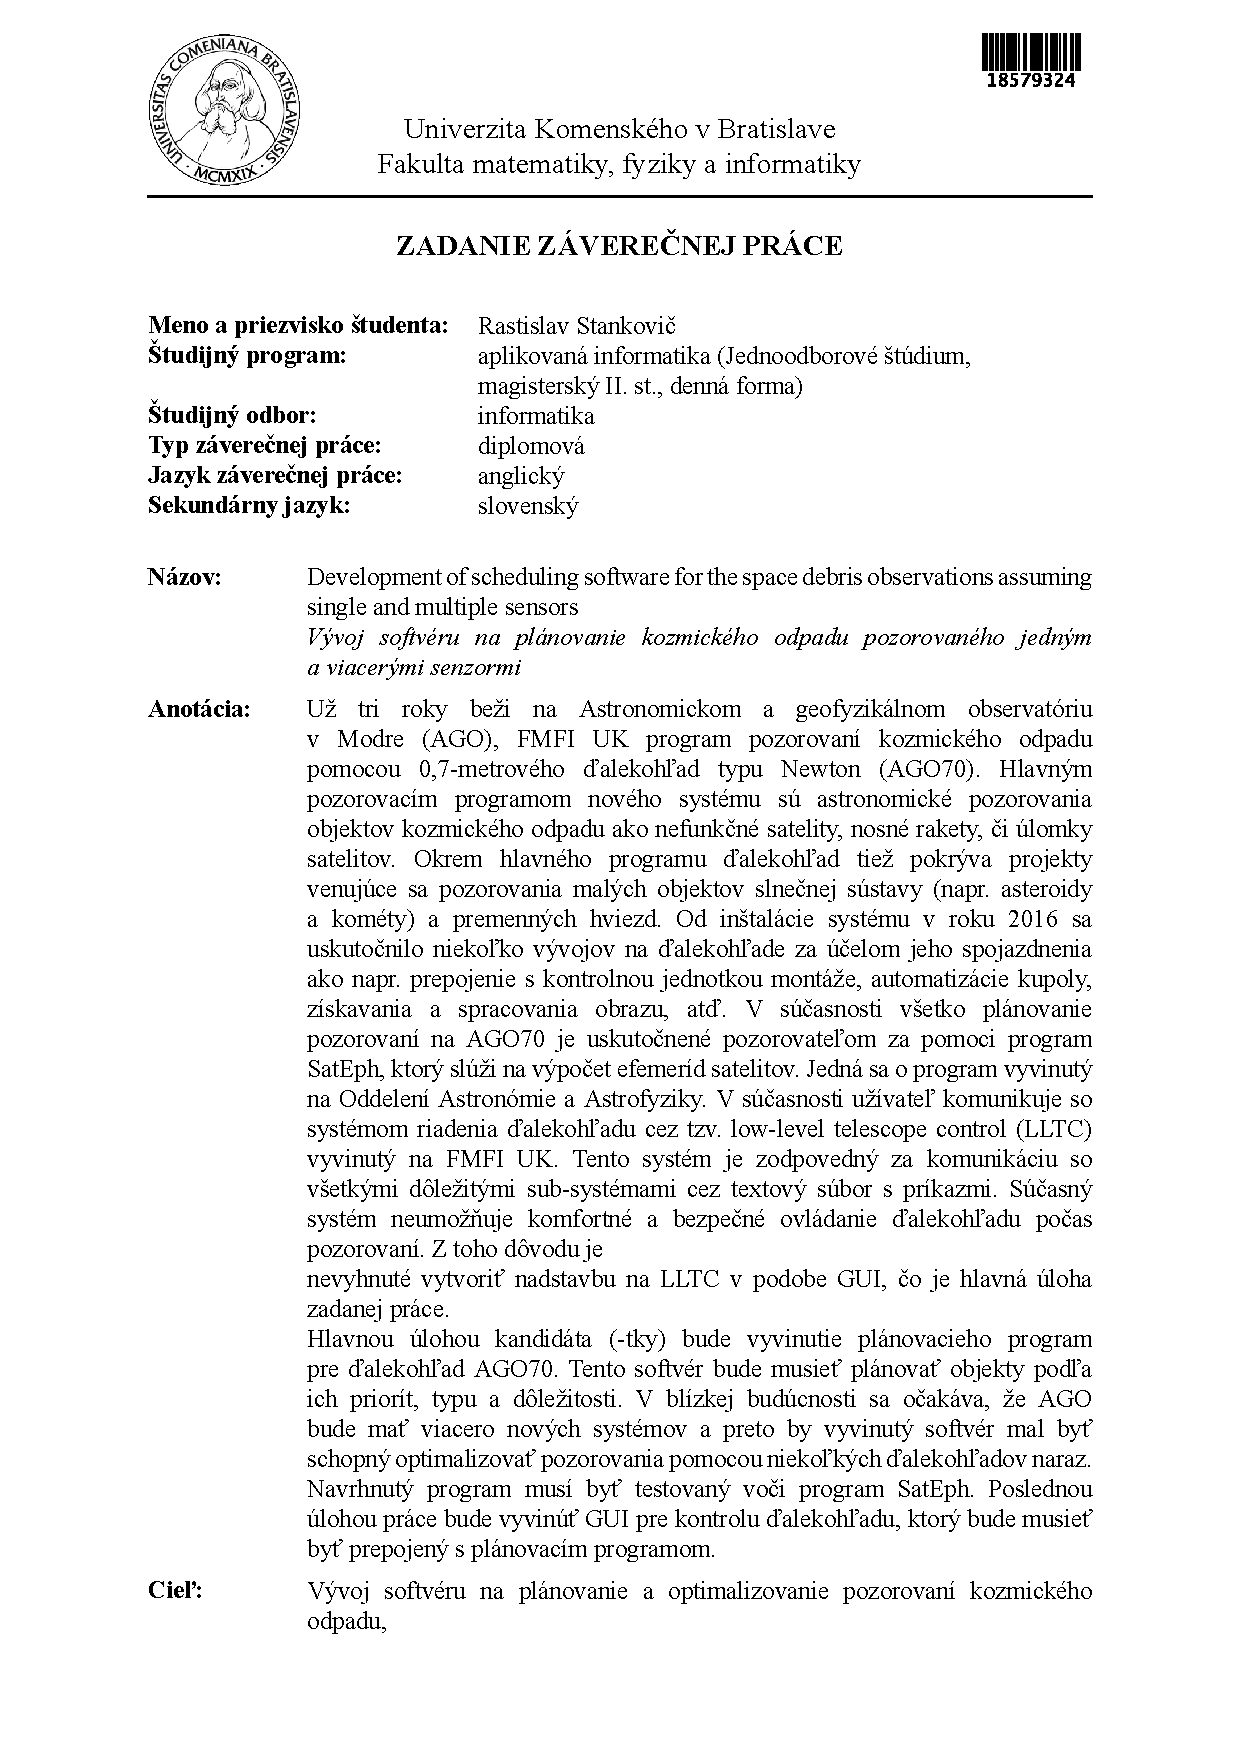
\includepdf[pages=-,pagecommand={},width=\textwidth]{images/ZadaniePrace}
{~}\vspace{12cm}

\noindent
Čestne prehlasujem, že som diplomovú prácu s názvom : \mftitle vypracoval samostnatne pod vedením môjho školiteľa a že som uviedol všetku použitú literatúru.
\newline \newline

\vfill
~ \hfill {\hbox to 6cm{\dotfill}} \\
\mfplacedate \hfill \mfauthor
\vfill\eject 
% koniec prehlasenia

\chapter*{Poďakovanie}\label{chap:thank_you}

\vfill\eject 
% koniec podakovania

\chapter*{Abstrakt}\label{chap:abstract_sk}
Táto diplomová práca sa zameriava na vytvorenie softvéru na plánovanie a optimalizovanie pozorovaní kozmického odpadu ako nefunkčných satelitov alebo ich úlomkov či nosných rakiet ďalekohľadmi AGO70 a inými súčasne, a následné vytváranie plánov budúcich pozorovaní. Jedná sa o nadstavbu existujúceho programu SatEph, ktorý nevyhovuje komfortným a bezpečným požiadavkám pre ovládanie. Hlavnou úlohou vytváraného softvéru je plánovať objekty podľa ich priorít, typu a dôležitosti v plánovacej časti programu za použitia ako sekvenčného, tak aj z časti prioritizovaného plánovania, ktorá je prepojená s GUI pre kontrolu ďalekohľadu používateľom softvéru. Priebeh testovania pred nasadením softvéru je uskutočnený vo vytvorenom emulátore, ktorý zahŕňa všetky funkcionality ďalekohľadov. Cieľom tejto diplomovej práce je vytvorenie funkčného softvéru, ktorého ovládanie je bezpečné a komfortné pre používateľa a ktorý správne vyhodnotí plánovacie aktivity pre ďalekohľady. 
~\\
Kľúčové slová: Plánovanie,vesmírny odpad, pozorovanie
\vfill\eject 

\chapter*{Abstract}\label{chap:abstract_en}
This master thesis focuses on the creation of software for planning and optimizing observations of space debris as non-functional satellites or their fragments or launch vehicles with AGO70 telescopes and others at the same time, and the subsequent creation of plans for future observations. It is an extension of the existing SatEph program, which does not meet the comfortable and safe requirements for control. The main task of the created software is to plan objects according to their priorities, type and importance in the planning part of the program using both sequential and part of prioritized planning, which is connected to the GUI for telescope control by software users. The testing process before software deployment is performed in the created emulator, which includes all the functionalities of the binoculars. The aim of this thesis is to create functional software, the control of which is safe and comfortable for the user and which correctly evaluates the planning activities for binoculars.

~\\
Keywords: scheduling,space debris,observation
\vfill\eject 
% koniec abstraktov

\tableofcontents

\mainmatter
% treba este prejst dokument ci je kod spravne formatovany
\input 01uvod.tex


\backmatter

\nocite{*}
\bibliographystyle{alpha}
\bibliography{references}

\listoffigures





\end{document}